\usepgfplotslibrary{groupplots}

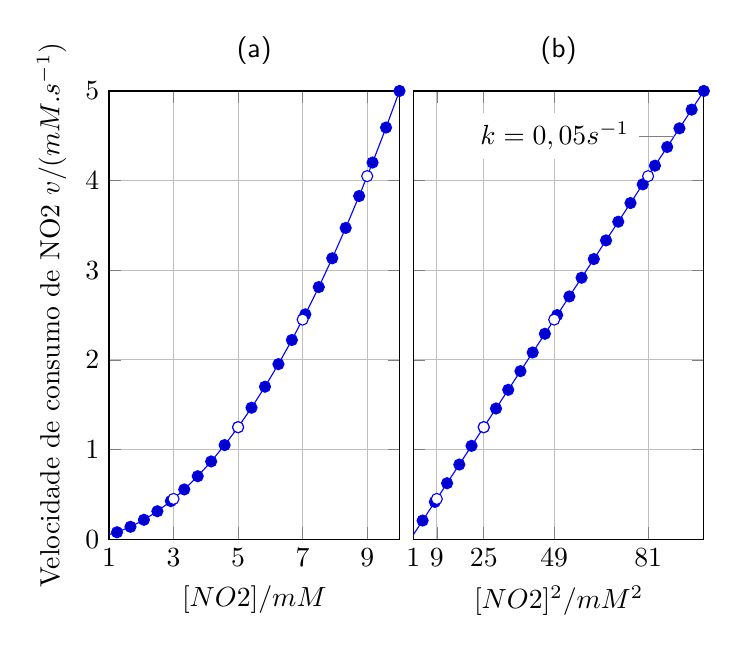
\begin{tikzpicture}
    \begin{groupplot}[
        group style={
            group size = 2 by 1,
            horizontal sep = 5pt,
            yticklabels at = edge left,
        },
        width = 150pt,
        height = 207pt,
        grid = major,
        ymin=0, ymax=5,
    ]

    \nextgroupplot 
        [
            title = {\sffamily (a)},
            ylabel = {Velocidade de consumo de \ce{NO2} $v/(\unit{mM.s^{-1}})$},
            xlabel = { $[\ce{NO2}]/\unit{mM}$ },
            xmin=1, xmax=10,
            domain = 0:10,
            xtick = {1, 3, 5, 7, 9},
        ]
        
        \addplot { 0.05*x^2 };
        
        \addplot 
            [
                mark=*, 
                color=blue, 
                mark options={fill=white},
                only marks,
            ] 
            coordinates
            { 
                (3, 0.45) 
                (5, 1.25)
                (7, 2.45)
                (9, 4.05)
            };
    
    \nextgroupplot
        [
            title = {\sffamily (b)},
            xmin=1, xmax=100,
            xlabel = { $[\ce{NO2}]^2/\unit{mM^2}$ },
            domain = 0:100,
            xtick = {1, 9, 25, 49, 81},
        ]
    
        \addplot { 0.05*x };
        
        \addplot 
            [
                mark=*, 
                color=blue, 
                mark options={fill=white},
                only marks,
            ] 
            coordinates
            { 
                (9, 0.45) 
                (25, 1.25)
                (49, 2.45)
                (81, 4.05)
            };

        \node[coordinate,pin={[fill=white] left:{$k = \qty{0,05}{s^{-1}}$}}] 
            at (axis cs:90, 4.5) {};
    \end{groupplot}
\end{tikzpicture}